\usetikzlibrary{calc}

\begin{frame}{this class: focus on Unix}
    \begin{itemize}
    \item Unix-like OSes will be our focus
    \item we have source code
    \item used to from 2150, etc.?
    \item have been around for a while
    \item xv6 imitates Unix
    \end{itemize}
\end{frame}

\begin{frame}{Unix history}
\vspace{-.5cm}
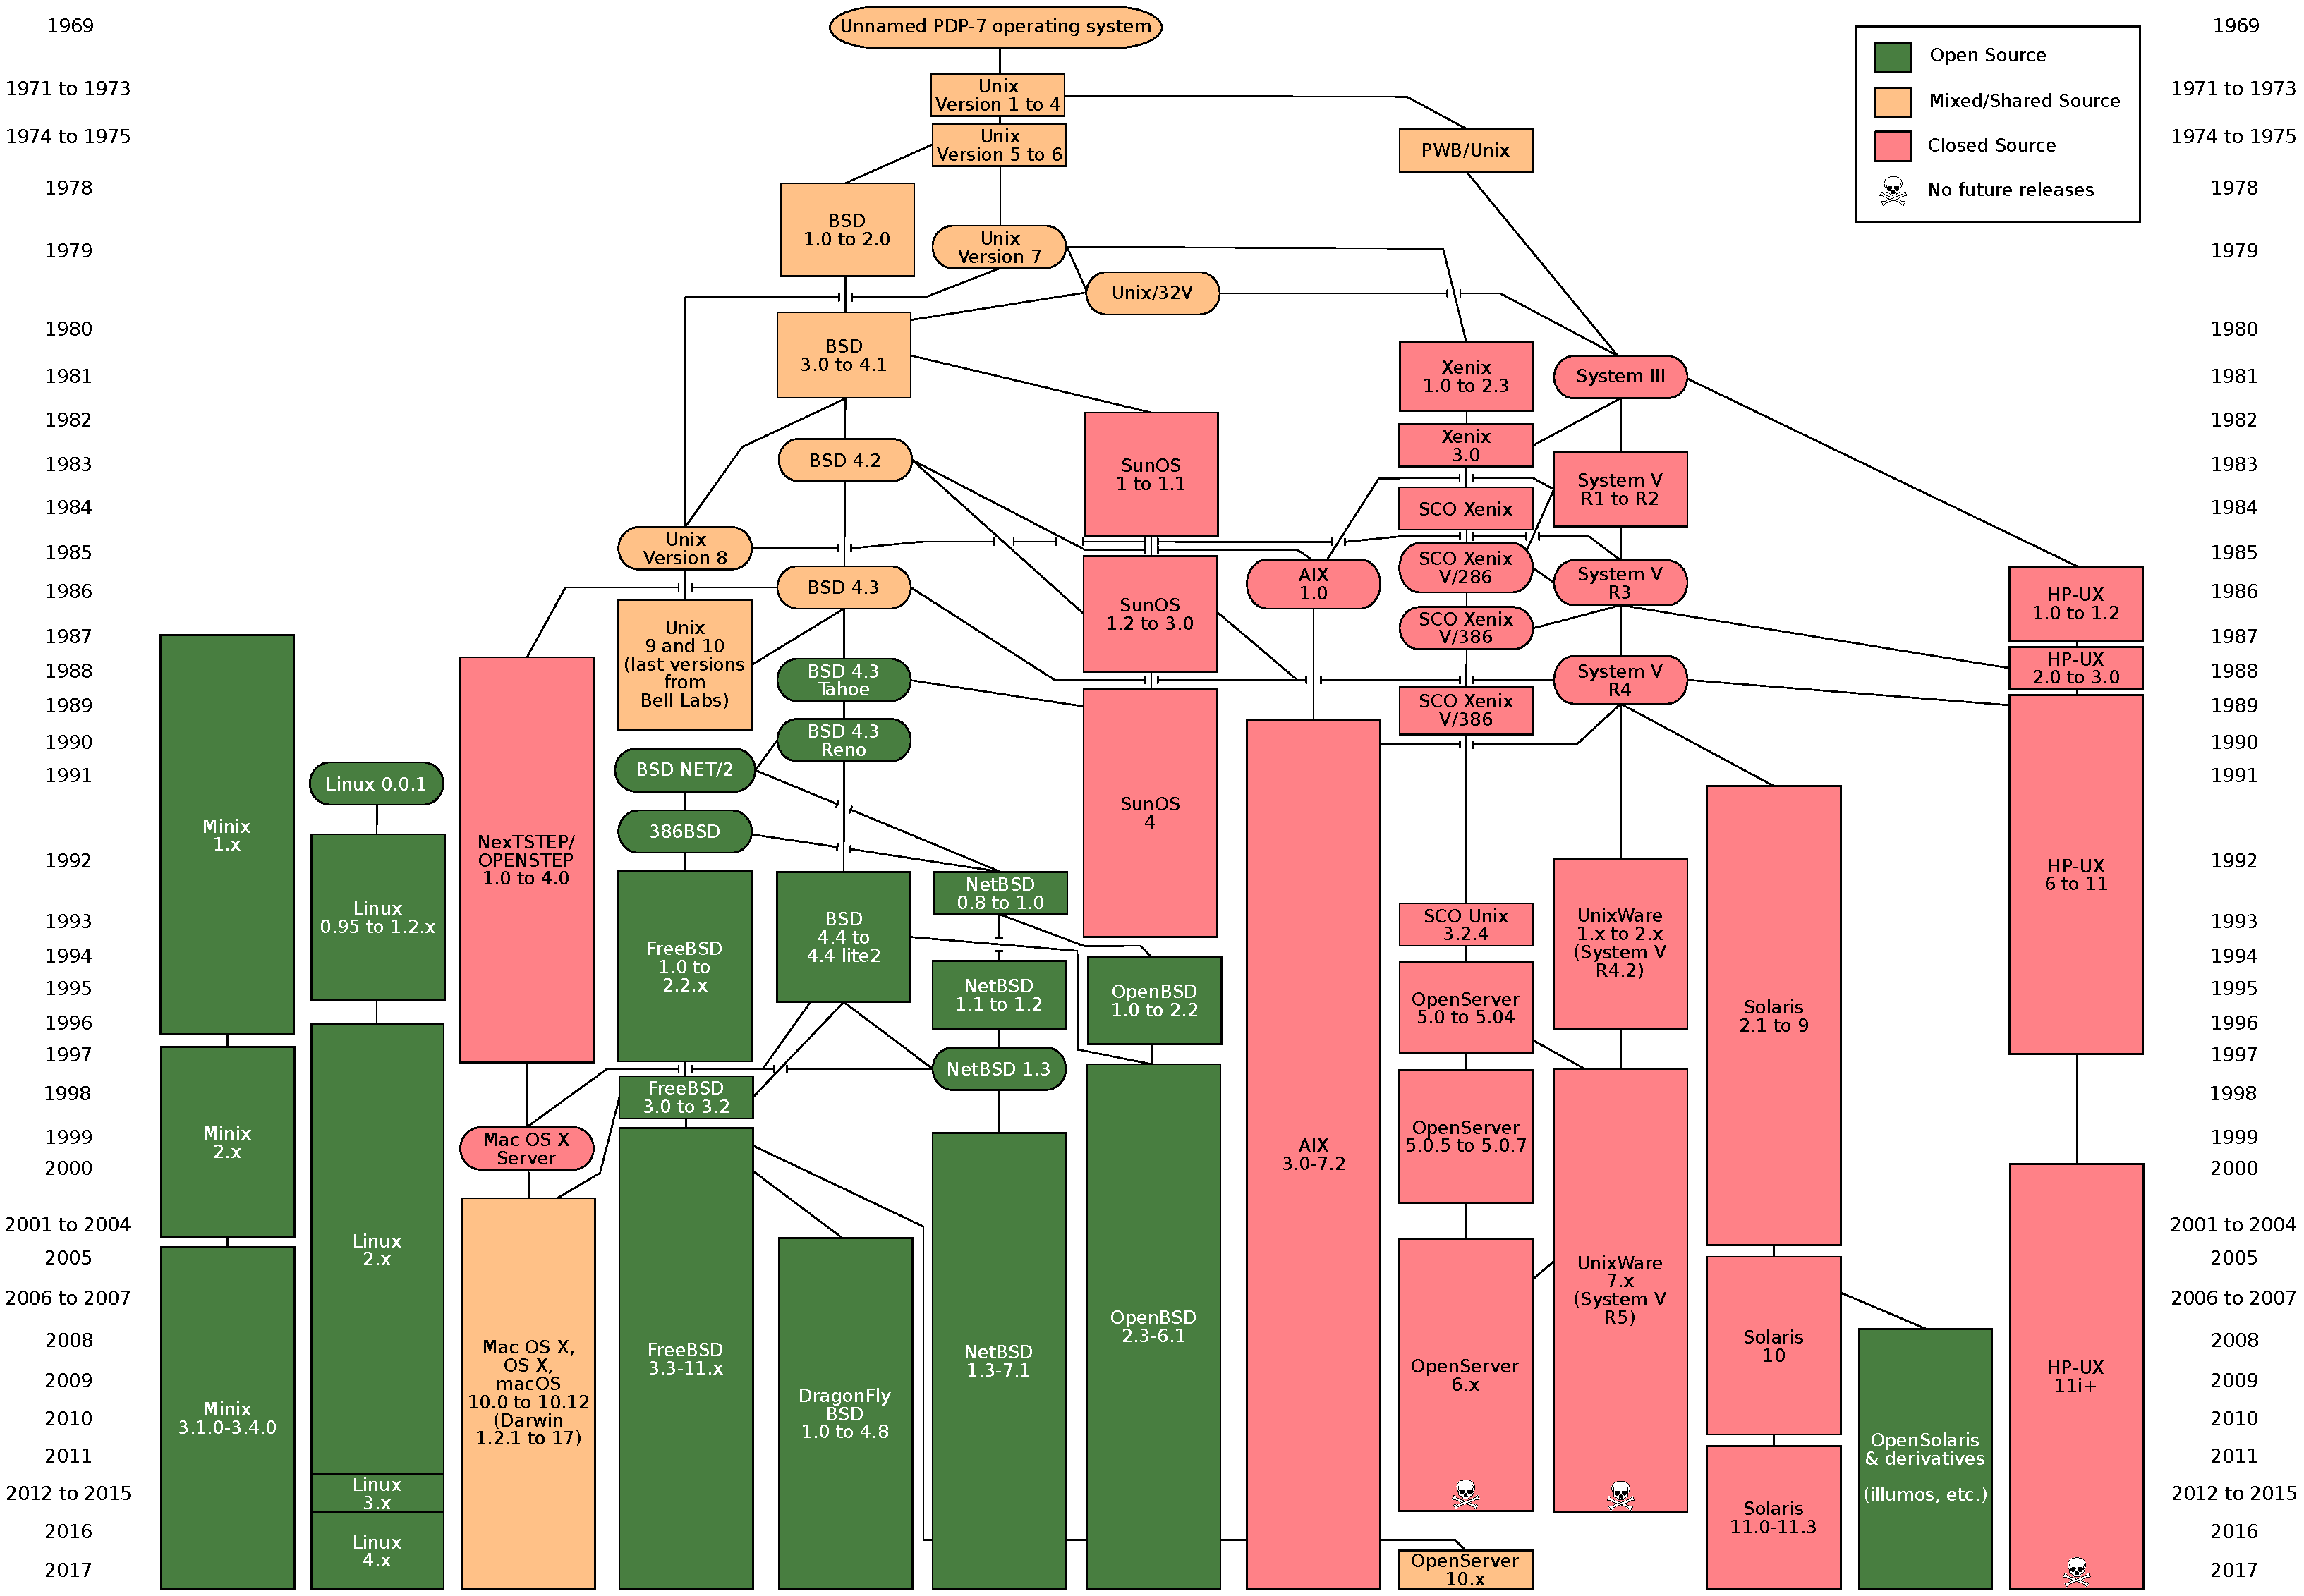
\includegraphics[height=0.9\textheight]{../unix-api/Unix_history-simple_en.pdf}
\imagecredit{image: Wikpedia/Eraserhead1+Infinity0+Sav\_vas}
\end{frame}

\begin{frame}{POSIX: standardized Unix}
\begin{itemize}
\item Portable Operating System Interface (POSIX) 
    \begin{itemize}
    \item ``standard for Unix''
    \end{itemize}
\item current version online: https://pubs.opengroup.org/onlinepubs/9699919799/
\item (almost) followed by most current Unix-like OSes
\item \ldots but OSes add extra features
\item \ldots and POSIX doesn't specify everything
\end{itemize}
\end{frame}

\begin{frame}{what POSIX defines}
\begin{itemize}
\item POSIX specifies the \myemph{library and shell interface}
    \begin{itemize}
    \item source code compatibility
    \end{itemize}
\item doesn't care what is/is not a system call\ldots
\item doesn't specify binary formats\ldots
\item idea: write applications for POSIX, recompile and run on all implementations
    \begin{itemize}
    \item this was a very important goal in the 80s/90s
    \item at the time, no dominant Unix-like OS (Linux was very immature)
    \end{itemize}
\end{itemize}
\end{frame}
